\section{Результати з математики}

Оглянемо отримані $122\ 026$ результатів, при цьому зауважимо, що чоловічих на $11\ 984$ більше за жіночих. 
Зобразимо гістограми результатів ЗНО з математики 2019 року для вибірки, наприклад, $10\ 000$ учнів:

\begin{figure}[H]
    \center{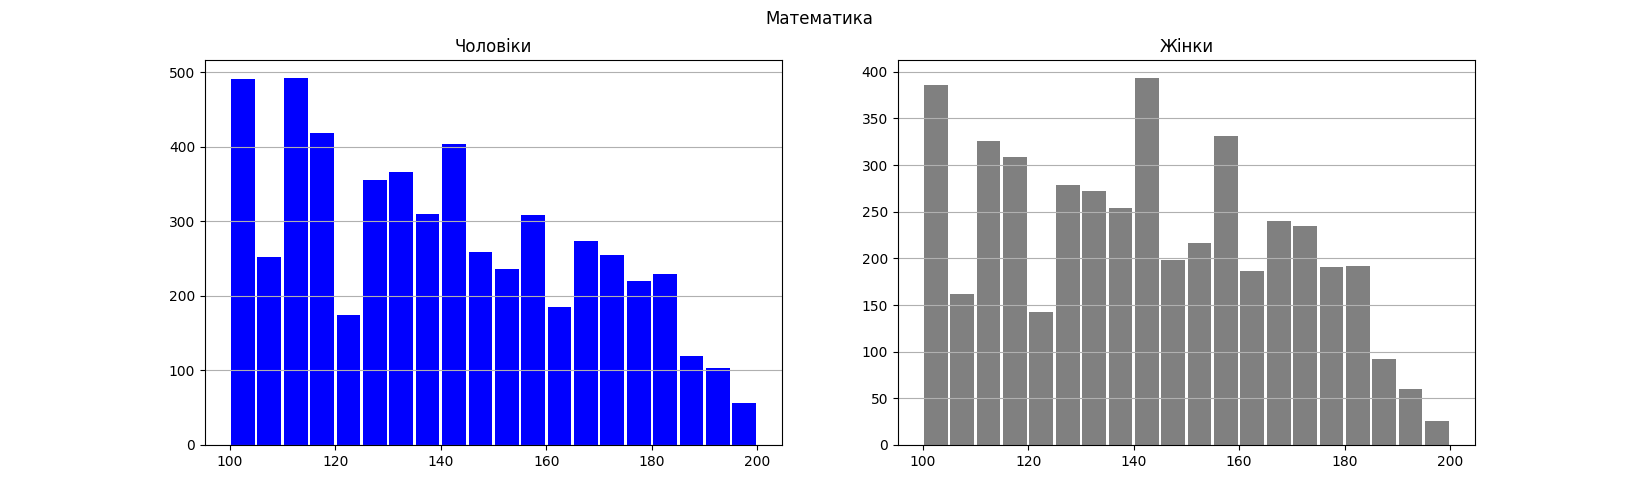
\includegraphics[trim=4cm 0cm 4cm 1cm, clip, width=1\linewidth]{MATH figures/MATH_10000.png}}
    \caption{Результати з математики}
    \label{figure: MATH initial data}
\end{figure}

З'ясуємо, чи відмінність між результатами з математики для жінок та чоловіків є статистично значущою.

\subsection{Перевірка гіпотези однорідності даних}

Нехай маємо дві незалежні вибірки $\left\{ X_i \right\}$ та $\left\{ Y_j \right\}$ однаково розподілених 
випадкових величин, розподіли $F_x$ й $F_y$ яких нам невідомі:
\begin{align*}
    &X_1 \ldots X_n\sim F_x && \text{результати чоловіків} \\
    &Y_1 \ldots Y_m\sim F_y && \text{результати жінок}
\end{align*}

Перевіримо гіпотезу про однорідність статистичного матеріалу, тобто гіпотезу, що ймовірності 
спостереження умовно високих, помірних та низьких балів в обох вибірках є однаковими. Таким чином 
матимемо $k=2$ вибірок, в яких елементи приймають $s=3$ різних значень. За аналогічних позначень 
гiпотеза перевiрки однорiдностi спосережуваних даних формулюватиметься так само, як і у 
виразах~(\ref{formula: hypothesis}):
\begin{align*}
    &\text{нульова гіпотеза} && H_0: p_{11}=p_{21},\ p_{12}=p_{22},\ p_{13}=p_{23} \\
    &\text{проти альтернативи} && H_1: \exists i,j\quad p_{1,j}\neq p_{2,j}
\end{align*}

А тоді критерієм перевірки гіпотези рівно як і у випадку обробки результатів з 
української мови (\ref{formula: criterion}) слугуватиме правило
\begin{equation*}
    \delta(x_1\ldots x_n,\ y_1\ldots y_m)=
    \begin{cases}
        H_1, & \rho\geqslant\chi^2_{1-\alpha;\ (k-1)(s-1)} \\
        H_0, & \rho<\chi^2_{1-\alpha;\ (k-1)(s-1)} \\
    \end{cases}
\end{equation*}

При цьому статистика критерію $\rho$ обчислюється аналогічно до формули (\ref{formula: criterion statistics}):
\begin{equation*}
    \rho\equiv \rho(x_1\ldots x_n,\ y_1\ldots y_m)=(n+m)\left( 
        \sum\limits_{i=1}^k \sum\limits_{j=1}^s \frac{\vartheta_{ij}^2}{\vartheta_{i\cdot}\vartheta_{\cdot j}} - 1 
        \right)
\end{equation*}

\subsubsection{Таблиця спостережуваних даних}

Складемо таблицю за спостережуваними даними навмання обраних $n=500$ та $m=500$ елементів із вибірок 
результатів ЗНО з математики для чоловіків та жінок:

\begin{table}[H]
    \vspace*{0.8cm}
    \begin{center}
        \begin{tabular}{|c||c|c|c|c|}
            \hline
             & \text{Низькі бали} & \text{Помірні бали} & \text{Високі бали} & \text{Всього} \\
            \hline \hline
            \text{Чоловіки} & 270 & 165 & 65 & 500 \\
            \hline
            \text{Жінки} & 268 & 174 & 58 & 500 \\
            \hline
            \text{Всього} & 538 & 339 & 123 & 1000 \\
            \hline
        \end{tabular}
        \caption{Таблиця спостережуваних значень з математики}
        \label{table: MATH homogeneity data}
    \end{center}
\end{table}

Обчислимо значення статистики критерію:
\begin{equation*}
    \rho = 1000\left( \frac{270^2}{538\cdot 500}+\frac{165^2}{339\cdot 500} + \ldots + 
    \frac{174^2}{339\cdot 500}+\frac{58^2}{123\cdot 500} - 1 \right) = 0.64
\end{equation*}

Водночас на рівні значущості $\alpha=0.01$ значення критичної точки
\begin{equation*} 
    \chi^2_{1-\alpha;\ (k-1)(s-1)}=\chi^2_{0.99;\ (2-1)(3-1)}=\chi^2_{0.99;\ 2}=9.21
\end{equation*}

\subsubsection{Висновок}

Оскільки значення статистики критерію є меншим за значення критичної точки, то згідно критерію гіпотеза 
про однорідність статистичних даних приймається. Отже, ймовірності спостереження оцінок різного рівня у 
вибірках для чоловіків та жінок, відповідно, є однаковими. Тобто стать ніяким чином не впливає на рівень 
отриманого балу.

\subsubsection*{Значення \texttt{p-value}}

Нехай випадкова величина $\tau$ має такий самий розподіл, як і статистика критерію й при цьому не залежить 
від неї: $\tau\sim\chi^2(2)$. Тоді величина \texttt{p-value} обчислюється як така ймовірність:
\[ P(\tau>\rho\ |\ H_0) = P(\tau>0.64) = 1-P(\tau\leqslant0.64) = 1-F_{\tau}(0.64) = 0.7261 \]

Тож для довільних значень $\alpha < \texttt{p-value}$ гіпотеза $H_0$ приймається.

\subsection{Перевірка гіпотези рівності дисперсій}

Маємо дві незалежні вибірки $\left\{ X_i \right\}$ та $\left\{ Y_j \right\}$ 
однаково розподілених випадкових величин, розподіли $F_x$ й $F_y$ яких нам невідомі:
\begin{align*}
    &X_1 \ldots X_n\sim F_x && \text{результати чоловіків} \\
    &Y_1 \ldots Y_m\sim F_y && \text{результати жінок}
\end{align*}

Проведемо нормалізацію даних крок за кроком, як це зображено на схемі (\ref{formula: normalization scheme}) 
розділу <<Нормалізація даних>>. У результаті отримаємо такі знормовні вибірки:
\begin{align*}
    &\overline{X^1}\ldots \overline{X^N}\sim N(\mu_x,\tfrac{1}{n}\sigma_x^2) && \text{середні результати чоловіків,} \\
    &\overline{Y^1}\ldots \overline{Y^N}\sim N(\mu_y,\tfrac{1}{n}\sigma_y^2) && \text{середні результати жінок,}
\end{align*}

при цьому
\[ \overline{X^i}=\frac{1}{n}\sum\limits_{j=1}^nX_j,\ 
   \overline{Y^i}=\frac{1}{n}\sum\limits_{j=1}^nY_j,\ i=\overline{1,N} \]

Побудуємо гістограми отриманих вибірок та переконаємося, що вони справді мають нормальний розподіл:

\begin{figure}[H]
    \center{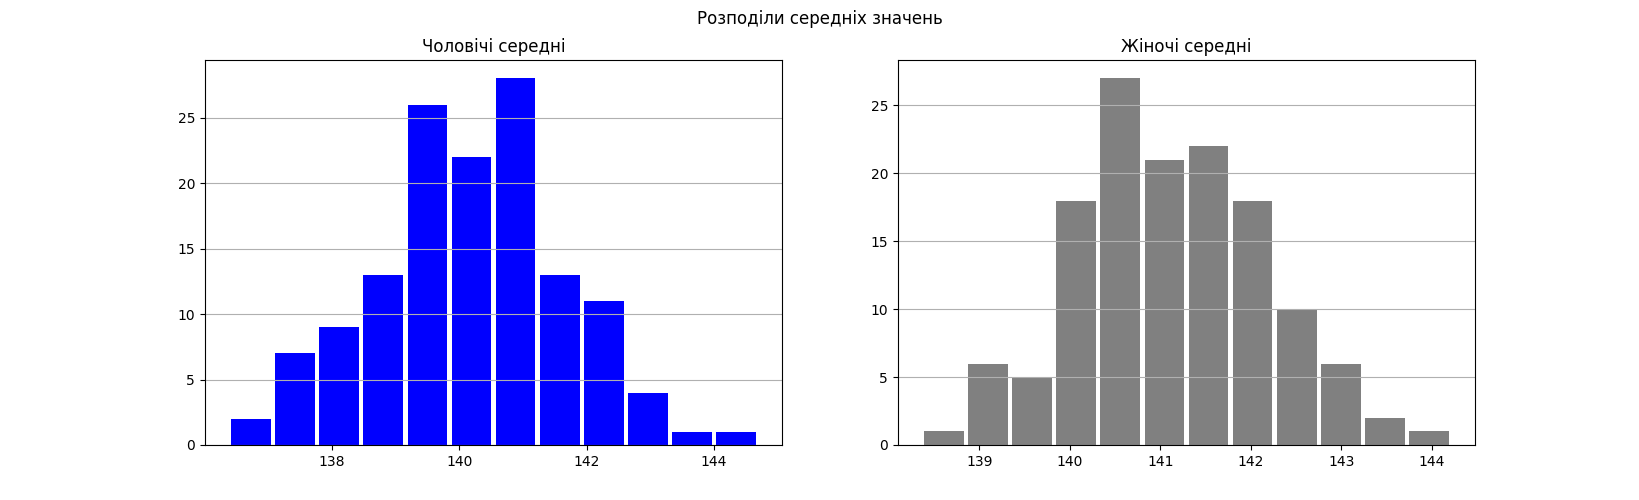
\includegraphics[trim=4cm 0cm 4cm 1cm, clip, width=1\linewidth]{MATH figures/Randomized_means_distribution_m400_N137_v4.png}}
    \caption{Гістограми наборів усереднених результатів ЗНО з математики}
    \label{figure: MATH means data}
\end{figure}

Як бачимо, криві в обох випадках мають схожі риси. Тож знову висунемо гiпотезу (\ref{formula: F-test hypothesis}) 
про рiвнiсть дисперсiй вибiрок результатiв чоловiкiв та жiнок:
\begin{align*}
    &\text{нульова гіпотеза} && H_0: \frac{\sigma_x^2}{\sigma_y^2}=1 \\
    &\text{проти альтернативи} && H_1: \frac{\sigma_x^2}{\sigma_y^2}\neq 1 \nonumber
\end{align*}

При істиності нульової гіпотези статистика критерію Фішера (\ref{formula: F-test statistic}) буде такою:
\begin{equation*}
    \rho\equiv
    \rho(\overline{ x^1}\ldots \overline{x^N},\ \overline{y^1}\ldots \overline{y^N})=\frac{S_Y^2}{S_X^2}
    \sim F\left( N-1,\ N-1 \right)
\end{equation*}

А критерієм перевірки гіпотези слугуватиме правило
\begin{equation*}
    \delta\equiv\delta(\overline{ x^1}\ldots \overline{x^N},\ \overline{y^1}\ldots \overline{y^N})=
    \begin{cases}
        H_1, & \rho\leqslant k^* \text{ або } \rho\geqslant k^{**} \\
        H_0, & \rho\in (k^*,\ k^{**}) \\
    \end{cases}\ ,
\end{equation*}

де значення критичних точок $k^*$ та $k^{**}$ при вказаному рівні значущості $\alpha$ є квантилями розподілу 
Фішера із $(N-1,\ N-1)$ степенями свободи (\ref{formula: F-test criterion values}):
\begin{align*}
    &k^* = f_{\frac{\alpha}{2};\ (N-1,\ N-1)} \\
    &k^{**} = f_{1-\frac{\alpha}{2};\ (N-1,\ N-1)}
\end{align*}

Розіб'ємо усю множину спостережуваних значень на $N=137$ неперетинних множин по $n=400$ елементів у кожній. 
У такому випадку статистична похибка обчислень є малою (детальніше -- на сторінці \pageref{page: MATH percentage point}). 
Наведемо потрібні величини для перевірки гіпотези рівності дисперсій у таблиці нижче:

\vspace{0.8cm}
\begin{table}[H]
    \begin{center}
        \begin{tabular}{||c|c|c|c|c|c||}
            \hline
            $n$ & $N$ & $\alpha$ & $S_X^2$ & $S_Y^2$ \\
            \hline \hline
            400 & 137 & 0.01 & 1.8055 & 1.4496 \\
            \hline
        \end{tabular}
        \caption{Значення шуканих параметрів F-тесту}
        \label{table: MATH F-test}
    \end{center}
\end{table}

Обчислимо значення статистики критерію:
\begin{equation*}
    \rho = \frac{S_Y^2}{S_X^2} = 0.8029
\end{equation*}

Водночас на рівні значущості $\alpha=0.01$ значення критичних точок
\begin{align*} 
   &k^* = f_{\frac{\alpha}{2};\ (N-1,\ N-1)} = f_{0.005;\ (136,\ 136)} = 0.6412 \\
   &k^{**} = f_{1-\frac{\alpha}{2};\ (N-1,\ N-1)} = f_{0.995;\ (136,\ 136)} = 1.5595
\end{align*}

\subsubsection{Висновок}
\label{page: MATH dispersion hypothesis}

Оскільки значення статистики критерію $\rho$ входить у проміжок $(0.6412,\ 1.5595)$, то згідно критерію 
на рівні значущості $\alpha=0.01$ нульова гіпотеза $H_0: \sigma_x^2=\sigma_y^2$ приймається. 
Для подільших міркувань введемо таке позначення: $\sigma_x^2=\sigma_y^2=\sigma^2$.

\newpage
\subsection*{Побудова довірчого інтервалу для різниці мат. сподівань}
\addcontentsline{toc}{subsection}{Побудова довірчого інтервалу для різниці математичних сподівань}

В результаті нормалізації початкових даних та перевірки гіпотези рівності дисперсій отримуємо такі дві вибірки: 
\begin{align}
    &\overline{X^1}\ldots \overline{X^N}\sim N(\mu_x,\tfrac{1}{n}\sigma^2) && \text{середні результати чоловіків,} \label{formula: MATH ND X} \\
    &\overline{Y^1}\ldots \overline{Y^N}\sim N(\mu_y,\tfrac{1}{n}\sigma^2) && \text{середні результати жінок,} \label{formula: MATH ND Y}
\end{align}

при цьому
\[ \overline{X^i}=\frac{1}{n}\sum\limits_{j=1}^nX^i_j,\ 
   \overline{Y^i}=\frac{1}{n}\sum\limits_{j=1}^nY^i_j,\ i=\overline{1,N} \]

Спробуємо оцінити, в якому інтервалі лежить значення різниці середніх балів для вибірок результатів ЗНО з 
математики чоловіків та жінок. Виконавши аналогічні перетворення, які наведенні на сторінці \pageref{page: seaching central statistic}, 
отримаємо шукану центральну статистику $G$ (\ref{formula: G central statistic}) для параметра $\theta=\mu_y-\mu_x:$
\begin{equation*}
    G=\left( (\overline{Y}-\overline{X})-\theta \right)\cdot \sqrt{\frac{N}{S_X^2+S_Y^2}}
    \sim t\left[ 2(N-1) \right]
\end{equation*}

Побудуємо довірчий інтервал рівня довіри $\gamma:$
\begin{equation*}
    \gamma \overset{\mathrm{def}}{=}P(g_1<G<g_2)=\int\limits_{g_1}^{g_2}f_G(x)\ dx
\end{equation*}

В силу симетричності розподілу Ст'юдента, найкоротший центральний довірчий інтервал матиме вид:
\begin{equation*}
    \gamma = P(g_1<G<g_2)=P(|\, G\, |<g),
\end{equation*}

де значення $g$ є квантилем рівня $\frac{1+\gamma}{2}$ розподілу Ст'юдента із $2(N-1)$ степенями свободи 
(Рис. \ref{figure: t interval}). Таким чином
\begin{equation}
    \gamma = P\left(
        -t_{\tfrac{1+\gamma}{2};\ 2(N-1)} < 
        \left((\overline{Y}-\overline{X})-\theta\right)\cdot \sqrt{\frac{N}{S_X^2+S_Y^2}} < 
        t_{\tfrac{1+\gamma}{2};\ 2(N-1)}
    \right) \label{formula: MATH trusted interval}
\end{equation}

Останнім кроком вкажемо конкретні значення усіх необхідних величин:

\vspace{0.8cm}
\begin{table}[H]
    \begin{center}
        \begin{tabular}{||c|c|c|c|c|c|c||}
            \hline
            $n$ & $N$ & $\gamma$ & $g=t_{0.975;\ 272}$ & $S_X^2$ & $S_Y^2$ & $\overline{Y}-\overline{X}$ \\
            \hline \hline
            400 & 137 & 0.95 & 1.97 & 1.8055 & 1.4496 & 0.9376 \\
            \hline
        \end{tabular}
        \caption{Значення параметрів для довірчого інтервалу різниці середніх}
        \label{table: MATH t interval}
    \end{center}
\end{table}

Підставивши у вираз (\ref{formula: MATH trusted interval}) значення, які наведені у таблиці вище, отримаємо такий довірчий 
інтервал для параметра $\theta=\mu_y-\mu_x$:
\begin{equation}
    P(0.63 < \theta < 1.24)=0.95 \label{formula: calculated MATH trusted interval}
\end{equation}

\subsubsection{Висновок}

Отримано довірчий інтервал рівня довіри $\gamma=0.95$ для величини різниці середніх значень 
оцінок з математики вибірок результатів чоловіків та жінок: $(0.63,\ 1.24)\ni \mu_y-\mu_x$. Хоча у 
вказаному проміжку немає нульового значення, тим не менш лівий кінець відрізку є близьким до $\{0\}$, що 
дає підстави перевірити гіпотезу про абсолютну нерозрізнюваність середніх. 

Так чи інакше, наразі можемо стверджувати, що при порівнянні результатів чоловіка та жінки оцінка з 
математики у жінки буде більшою за оцінку у чоловіка на бал у $0.94\pm 0.3$ пункти, при цьому в середньому 
у п'яти зі ста таких порівнянь вказане наближення може бути хибним.

\subsection{Перевірка гіпотези рівності математичних сподівань}

Нехай задано дві незалежні нормально розподілені вибірки (\ref{formula: MATH ND X})-(\ref{formula: MATH ND Y}) 
із невідомими математичними сподіваннями та невідомими, проте однаковими дисперсіями: 
\begin{align*}
    &\overline{X^1}\ldots \overline{X^N}\sim N(\mu_x,\tfrac{1}{n}\sigma^2) && \text{середні результати чоловіків} \\
    &\overline{Y^1}\ldots \overline{Y^N}\sim N(\mu_y,\tfrac{1}{n}\sigma^2) && \text{середні результати жінок}
\end{align*}

Перевіримо гіпотезу рівності математичних сподівань:
\begin{align*}
    &\text{нульова гіпотеза} && H_0: \mu_y=\mu_x \\
    &\text{проти односторонньої альтернативи} && H_1: \mu_y>\mu_x 
\end{align*}

Або в еквівалентному записі:
\begin{align}
    &\text{нульова гіпотеза} && H_0: \mu_y-\mu_x=0 \label{formula: mathematical expectation equivalence hypothesis} \\
    &\text{проти односторонньої альтернативи} && H_1: \mu_y-\mu_x>0 \nonumber
\end{align}

Скористаємося побудованою у попередньому розділі статистикою (\ref{formula: G central statistic}). При істиності 
нульової гіпотези $H_0: \mu_y-\mu_x=0$ отримаємо таку статистику критерію:
\begin{equation}
    \rho\equiv\rho(\overline{ x^1}\ldots \overline{x^N},\ \overline{y^1}\ldots \overline{y^N})=
    (\overline{Y}-\overline{X}) \cdot \sqrt{\frac{N}{S_X^2+S_Y^2}}
    \sim t\left[ 2(N-1) \right] \label{formula: mathematical expectation equivalence statistic}
\end{equation}

Тоді перевищення цією статистикою певного критичного значення формуватиме критичну область нульової 
гіпотези. Як наслідок критерієм перевірки гіпотези слугуватиме правило
\begin{equation}
    \delta\equiv\delta(\overline{ x^1}\ldots \overline{x^N},\ \overline{y^1}\ldots \overline{y^N})=
    \begin{cases}
        H_1, & \rho\geqslant k \\
        H_0, & \rho < k \\
    \end{cases} \label{formula: mathematical expectation equivalence criterion}
\end{equation}

Значення критичної точки $k$ знайдемо з означення помилки першого роду: 
\begin{equation*}
    \alpha\overset{\mathrm{def}}{=}P(\delta\in K_{\alpha}\ |\ H_0)=P(\rho \geqslant k\ |\ H_0)=1-F_t(k)
\end{equation*}

Таким чином $k$ є квантилем розподілу Ст'юдента із $\left[ 2(N-1) \right]$ степенями свободи при вказаному 
рівні значущості $\alpha$:
\begin{equation}
    k=t_{1-\alpha;\ 2(N-1)} \label{formula: mathematical expectation equivalence criterion values}
\end{equation}

Скористаємося наведеними у Табл. \ref{table: MATH t interval} значеннями для перевiрки гiпотези рiвностi 
математичних сподівань. Обчислимо значення статистики критерію:
\begin{equation*}
    \rho = (\overline{Y}-\overline{X}) \cdot \sqrt{\frac{N}{S_X^2+S_Y^2}} = 6.0827
\end{equation*}

Водночас на рівні значущості $\alpha=0.01$ значення критичної точки
\begin{equation*} 
   k = t_{1-\alpha;\ 2(N-1)} = t_{0.99;\ 272} = 2.34
\end{equation*}

\subsubsection{Висновок}

Оскільки значення статистики критерію перевищує критичну точку, то згідно критерію 
(\ref{formula: mathematical expectation equivalence criterion}) на рівні значущості $\alpha=0.01$ нульова 
гіпотеза $H_0: \mu_y=\mu_x$ відхиляється. Більш того, при спробі обчислити \texttt{p-value} натикаємося на 
невиправдано малі значення $\alpha$, при яких гіпотеза $H_0$ приймалася б. Отже, навіть попри близькість 
лівого кінця довірчого інтервалу (\ref{formula: calculated MATH trusted interval}) до нуля, цією межою не 
можна знехтувати.

\subsection{Побудова довірчого інтервалу для значення дисперсії}

Наостанок віднайдемо проміжок можливих значень дисперсії нормованих вибірок. В силу прийняття гіпотези 
рівності дисперсій (сторінка \pageref{page: MATH dispersion hypothesis}) із оригінальних наборів
\begin{align*}
    &\overline{X^1}\ldots \overline{X^N}\sim N(\mu_x,\tfrac{1}{n}\sigma^2) && \text{середні результати чоловіків} \\
    &\overline{Y^1}\ldots \overline{Y^N}\sim N(\mu_y,\tfrac{1}{n}\sigma^2) && \text{середні результати жінок}
\end{align*}

аналогічними кроками, як це виконано на сторінці \pageref{page: seaching central statistic}, можна сформувати 
випадкову величину (\ref{formula: eta}) розподілу хі-квадрат із $\left[ 2(N-1) \right]$ степенями свободи, 
при цьому для параметра дисперсії $\frac{1}{n}\sigma^2$ ця величина відіграватиме роль центральної статистики:
\begin{equation}
    G\equiv\frac{(N-1)}{\sigma^2/n}\left( S_X^2+S_Y^2 \right)\sim \chi^2\left[ 2(N-1) \right]
\end{equation}

А тоді довірчий інтервал рівня довіри $\gamma$ матиме вид:
\begin{equation}
    \gamma \overset{\mathrm{def}}{=} P(g_1<G<g_2)=\int\limits_{g_1}^{g_2}f_G(x)\ dx
\end{equation}

Значення $g_1$ та $g_2$, як це показано на Рис. \ref{figure: chi interval}, є квантилями рівнів 
$\frac{1-\gamma}{2}$ та $\frac{1+\gamma}{2}$ розподілу хі-квадрат із $\left[ 2(N-1) \right]$ степенями свободи:
\begin{equation*}
    g_1=\chi^2_{\tfrac{1-\gamma}{2};\ 2(N-1)},\  
    g_2=\chi^2_{\tfrac{1+\gamma}{2};\ 2(N-1)}   
\end{equation*}

Підставляючи отримані результати, матимемо:
\begin{equation}
    \gamma = P\left( 
        \chi^2_{\tfrac{1-\gamma}{2};\ 2(N-1)} < 
        \frac{(N-1)}{\sigma^2/n}\left( S_X^2+S_Y^2 \right) < 
        \chi^2_{\tfrac{1+\gamma}{2};\ 2(N-1)} 
    \right) \label{formula: MATH chi trusted interval}
\end{equation}

Наостанок вкажемо конкретні значення усіх необхідних величин:

\vspace{0.8cm}
\begin{table}[H]
    \begin{center}
        \begin{tabular}{||c|c|c|c|c|c|c||}
            \hline
            $n$ & $N$ & $\gamma$ & $g_1=\chi^2_{0.025;\ 272}$ & $g_2=\chi^2_{0.975;\ 272}$ & $S_X^2$ & $S_Y^2$ \\
            \hline \hline
            400 & 137 & 0.95 & 228.21 & 319.58 & 1.8055 & 1.4496 \\
            \hline
        \end{tabular}
        \caption{Значення параметрів для довірчого інтервалу дисперсії}
        \label{table: MATH chi interval}
    \end{center}
\end{table}

Підставивши у вираз (\ref{formula: MATH chi trusted interval}) наведені вище значення, отримаємо 
такий довірчий інтервал для параметра $\frac{1}{n}\sigma^2:$
\begin{equation*}
    P(1.39\ < \frac{\sigma^2}{n} <\ 1.94)=0.95
\end{equation*}

\subsubsection{Висновок}

Таким чином для сформованих нормально розподілених вибірок (\ref{formula: MATH ND X})-(\ref{formula: MATH ND Y}) 
значення дисперсії в середньому лише у п'яти елементів вибірки зі ста буде виходити за межі проміжку від $1.39$ 
до $1.94$ балів.

\subsection{Статистична похибка обчислень}
\label{page: MATH percentage point}

Статистичною похибкою обчислень називатимемо найменшу величину $\Delta$ відхилення різниці вибіркових 
середніх від істинного значення різниці математичних сподівань заданих вибірок 
(\ref{formula: MATH ND X})-(\ref{formula: MATH ND Y}) з щонайменшою ймовірністю у $95\%$. 
Тобто шукана похибка $\Delta$ обчислюватиметься як така ймовірність:
\begin{equation*}
    P\left(\ \left| (\overline{Y}-\overline{X})-(\mu_y-\mu_x) \right| \leqslant \Delta\ \right)\geqslant 0.95
\end{equation*}

Виконавши аналогічні міркування, які наведені на сторінці \pageref{page: UKR percentage point}, отримаємо, 
що величина похибки $\Delta$ виражатиметься через квантиль рівня $0.975$ розподілу Ст'юдента з 
$\left[ 2(N-1) \right]$ степенями свободи:
\begin{equation}
    \Delta \geqslant t_{0.975;\ 2(N-1)} \cdot \sqrt{\frac{S_X^2+S_Y^2}{N}}
\end{equation}

Таблиця необхідних значень виглядатиме таким чином:

\vspace{0.8cm}
\begin{table}[H]
    \begin{center}
        \begin{tabular}{||c|c|c|c||}
            \hline
            $N$ & $t_{0.975;\ 272}$ & $S_X^2$ & $S_Y^2$ \\
            \hline \hline
            137 & 1.97 & 1.8055 & 1.4496 \\
            \hline
        \end{tabular}
        \caption{Значення параметрів для обчислення статистичної похибки}
        \label{table: MATH percentage point}
    \end{center}
\end{table}

Тож остаточно найменша величина відхилення $\Delta = 0.3$, а тоді початкова ймовірнісна нерівність матиме вид:
\begin{equation*}
    P\left(\ \left| (\overline{Y}-\overline{X})-(\mu_y-\mu_x) \right| \leqslant 0.3\ \right)\geqslant 0.95
\end{equation*}

\subsubsection{Висновок}

Для встановлених значень $n=400$ й відповідно $N=137$ статистична похибка відхилення різниці вибіркових 
середніх від істинного значення різниці математичних сподівань складає $\Delta = 0.3$ бала з ймовірністю, 
більшою за $95\%$. Можемо стверджувати, що обчислення за такого значення похибки мають високу точність, 
оскільки величина $\Delta = 0.3$ є лише $0.15\%$ від можливих $200$ балів за результат тесту.